\newpage
\section{Exploration and Analysis}
    \subsection{What makes a movie successful?}
        % We would like you to explore what makes a movie popular and/or successful.
        \begin{multicols}{2}
            \paragraph{}
                In order to ascertain which factors are most influential in determining the
                    success of a movie, it is necessary to first define what constitutes success.
                For the purpose of this analysis, success is defined as the movie's revenue.
                By examining the correlations between the movie's revenue and other factors, we
                    can gain insight into which factors have the greatest impact on the success of
                    a movie.
                These correlations are visualised in Figure~\ref{fig-heatmap}.

                \begin{figure}[H]
                    \centering
                    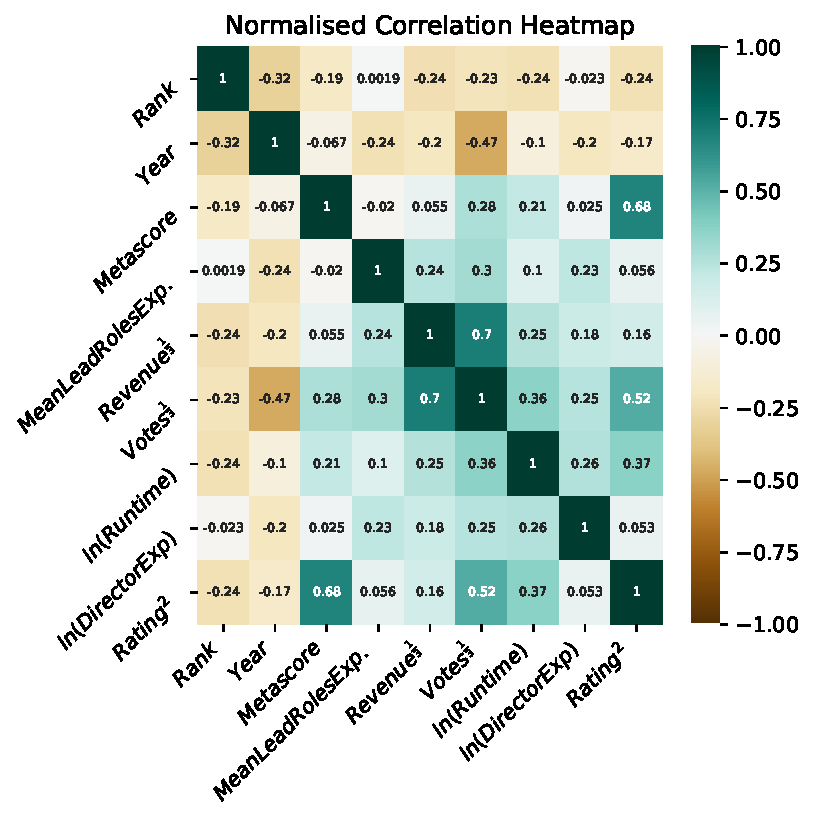
\includegraphics[width=\linewidth]{Final/Normalised Correlation Heatmap.pdf}
                    \caption{
                        A heatmap illustrating the strength of correlations (using PMCC) between various normalised
                        variables from the IMDb dataset~\cite{data:IMDb} and the TMD
                        data~\cite{data:TMD}.
                    }\label{fig-heatmap}
                \end{figure}

                \begin{figure}[H]
                    \centering
                    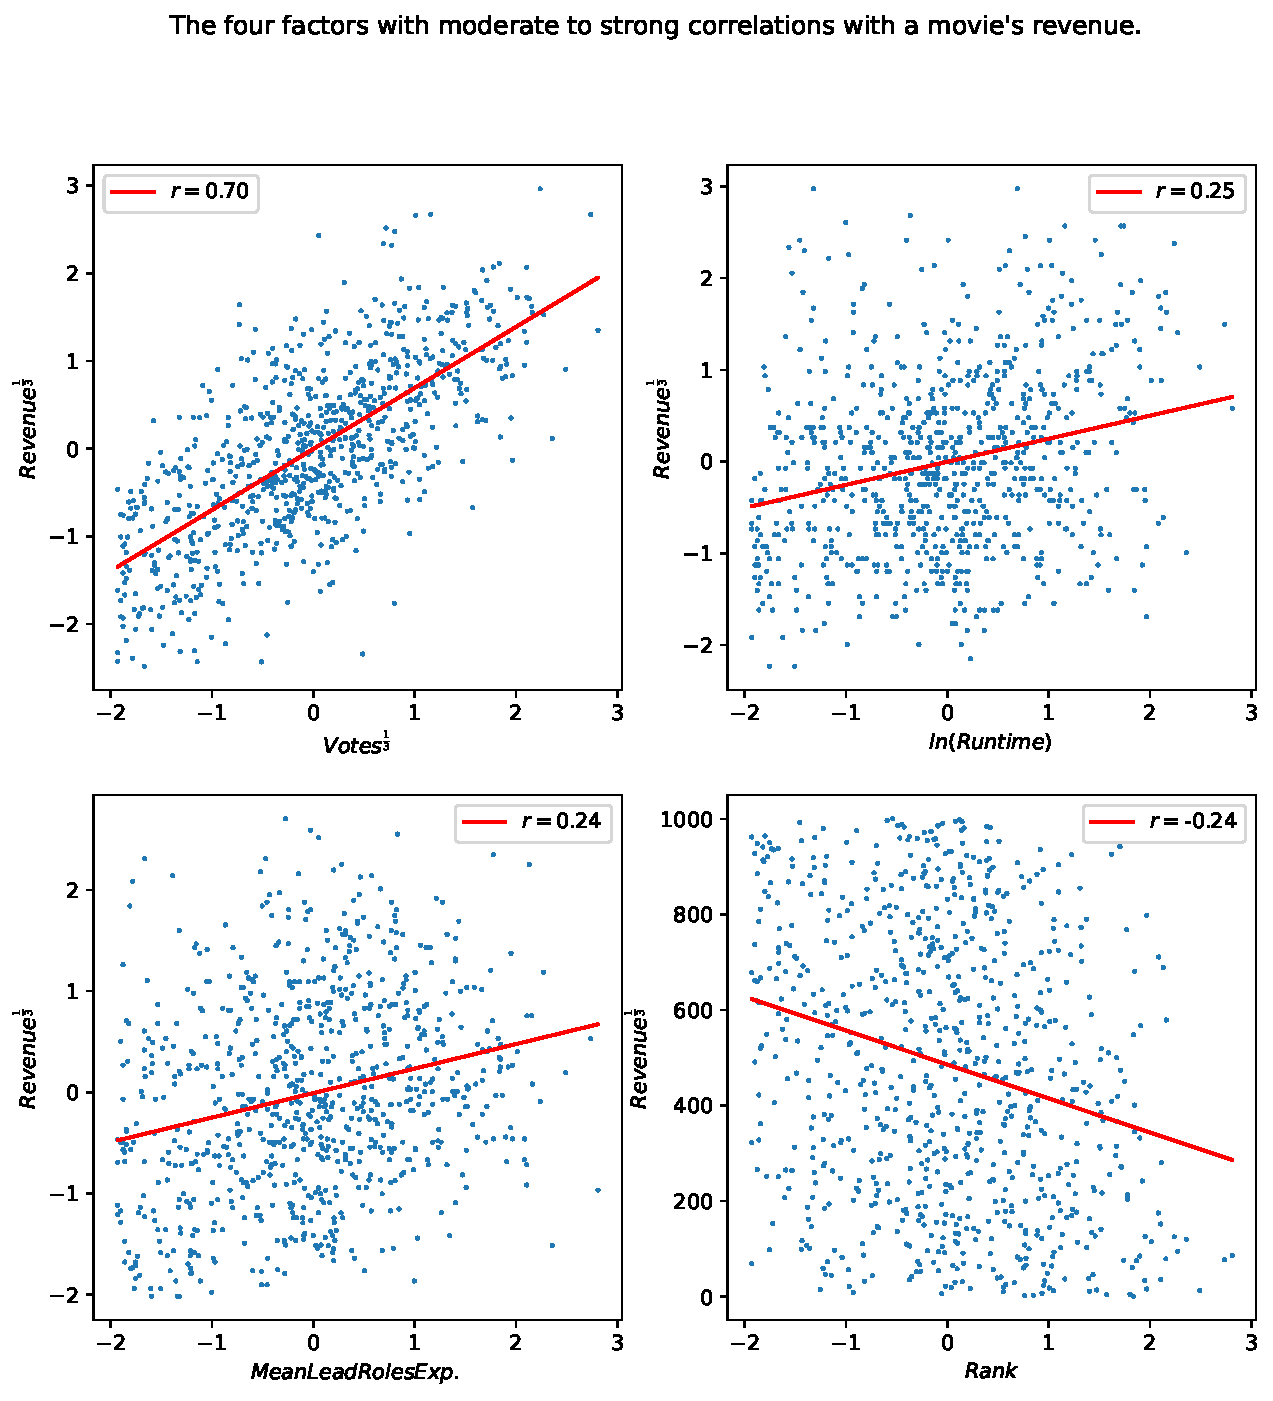
\includegraphics[width=\linewidth]{Final/Revenue Factors.pdf}
                    \caption{
                        Scatter plots showing the relationships between a movie's revenue and the four
                        factors with moderate or strong correlations.
                    }\label{fig-revenue-factors}
                \end{figure}

            \paragraph{}
                Figure~\ref{fig-heatmap} reveals a strong positive correlation (0.7) between a
                    movie's revenue and the number of votes it receives on IMDb, suggesting that
                    the more votes a movie receives, the higher its revenue is likely to be.
                Additionally, the heatmap shows moderate positive correlations between the
                    movie's revenue and its runtime (0.25) and between the movie's revenue and the
                    experience of the actors in lead roles (0.24), indicating that longer runtimes
                    and more experienced actors may be associated with higher revenues.
                In contrast, there is a moderate negative correlation between a movie's revenue
                    and its rank on IMDb (-0.24), suggesting that higher ranks on IMDb do not
                    necessarily translate to higher revenues.
                These four correlations are shown in more detail in
                    Figure~\ref{fig-revenue-factors}.
        \end{multicols}

    \subsection{The relationship between a movie's ranked position and its number of votes}
        % We would also like you to visualise the distribution of ranked position and
        % number of votes, and comment on the relationship between them.

    \subsection*{}
        \paragraph{}

            % Suggested 500 words for individual report; proportionately longer for group
            % projects). 

            % Revenue Multiple Regression
            In order to further analyze the correlations between the various movie details
                and the revenue they generated, we created a multiple regression model using
                the normalized data we collected.
            The target variable was the normalised revenue, with the rest of the dataset as
                the predictor variables, excluding Genre and Title.
            $Votes^\frac{1}{3}$ was excluded as it is causally linked to Revenue; the more votes, the more people bought movie tickets.
            The model uses Ordinary Least Squares regression and a constant column has been
                added to show y-intercept.
            The summary results are provided below.
            \begin{table}[H]
                \begin{center}
                    \begin{tabular}{lclc}
                        \toprule
                        \textbf{Dep.~Variable:}    & $Revenue^{\frac{1}{3}}$ & \textbf{  R-squared:         } & 0.404    \\
                        \textbf{Model:}            & OLS                     & \textbf{  Adj.~R-squared:    } & 0.393    \\
                        \textbf{Method:}           & Least Squares           & \textbf{  F-statistic:       } & 36.60    \\
                        \textbf{No.~Observations:} & 826                     & \textbf{  AIC:               } & 1921.    \\
                        \textbf{Df Residuals:}     & 810                     & \textbf{  BIC:               } & 1996.    \\
                        \textbf{Df Model:}         & 15                      & \textbf{  Prob (F-statistic):} & 1.35e-80 \\
                        \textbf{Covariance Type:}  & nonrobust               & \textbf{  Log-Likelihood:    } & -944.32  \\
                        \bottomrule
                    \end{tabular}
                    \begin{tabular}{lcccccc}
                                                        & \textbf{coef} & \textbf{std err} & \textbf{t} & \textbf{P$> |$t$|$} & \textbf{[0.025} & \textbf{0.975]} \\
                        \midrule
                        \textbf{$const$}                & 114.0116      & 19.712           & 5.784      & 0.000               & 75.319          & 152.705         \\
                        \textbf{$Rank$}                 & -0.0006       & 0.000            & -5.654     & 0.000               & -0.001          & -0.000          \\
                        \textbf{$Year$}                 & -0.0565       & 0.010            & -5.770     & 0.000               & -0.076          & -0.037          \\
                        \textbf{$Metascore$}            & 0.0416        & 0.038            & 1.093      & 0.275               & -0.033          & 0.116           \\
                        \textbf{$Mean Lead Roles Exp.$} & 0.1125        & 0.030            & 3.793      & 0.000               & 0.054           & 0.171           \\
                        \textbf{$ln(Runtime)$}          & 0.1705        & 0.033            & 5.203      & 0.000               & 0.106           & 0.235           \\
                        \textbf{$ln(Director Exp)$}     & 0.0507        & 0.029            & 1.756      & 0.079               & -0.006          & 0.107           \\
                        \textbf{$Rating^2$}             & 0.0816        & 0.041            & 2.013      & 0.044               & 0.002           & 0.161           \\
                        \textbf{$Action$}               & 0.1824        & 0.070            & 2.598      & 0.010               & 0.045           & 0.320           \\
                        \textbf{$Adventure$}            & 0.4765        & 0.074            & 6.452      & 0.000               & 0.332           & 0.621           \\
                        \textbf{$Sci-Fi$}               & 0.0318        & 0.087            & 0.364      & 0.716               & -0.140          & 0.203           \\
                        \textbf{$Thriller$}             & -0.0395       & 0.078            & -0.504     & 0.615               & -0.193          & 0.114           \\
                        \textbf{$Comedy$}               & 0.1145        & 0.072            & 1.599      & 0.110               & -0.026          & 0.255           \\
                        \textbf{$Drama$}                & -0.5579       & 0.071            & -7.877     & 0.000               & -0.697          & -0.419          \\
                        \textbf{$Romance$}              & -0.0243       & 0.084            & -0.288     & 0.773               & -0.190          & 0.141           \\
                        \textbf{$Crime$}                & -0.0545       & 0.082            & -0.664     & 0.507               & -0.216          & 0.107           \\
                        \bottomrule
                    \end{tabular}
                    \begin{tabular}{lclc}
                        \textbf{Omnibus:}       & 2.065  & \textbf{  Durbin-Watson:     } & 2.048    \\
                        \textbf{Prob(Omnibus):} & 0.356  & \textbf{  Jarque-Bera (JB):  } & 1.964    \\
                        \textbf{Skew:}          & -0.055 & \textbf{  Prob(JB):          } & 0.375    \\
                        \textbf{Kurtosis:}      & 2.788  & \textbf{  Cond.~No.          } & 1.53e+06 \\
                        \bottomrule
                    \end{tabular}
                    %\caption{OLS Regression Results}
                \end{center}

                \caption[short]{Multiple Regression results summary}\label{tab:revenue-ols-summary}
            \end{table}
            This model performs respectably, explaining about 40\% of the variance in user
                ratings.
            It is also statistically significant, getting a very small $P(F-statistic)$.
            This indicates that the revenue of a movie can be predicted from the data
                present in the dataset, albeit not extremely well.
            However, the relatively good $R^2$ value does indicate a well performing model,
                as such we can postulate that at least some of these factors are impactful on
                the revenue a movie makes.
            There are also a few interesting observations that can be made about this data.

            % Director vs Actor for selling tickets
            One such observation is that the experience of lead actors has a statistically
                significant effect on movie ticket sales (p<0.05), while the experience of
                directors does not (p>0.05).
            This raises the question of whether the director has as much of an impact as
                the actors when it comes to selling tickets.
            A possible explanation is the fact that promotional posters for movies often
                focus on the actors~\cite{label}, with their faces being the first thing a
                consumer sees.
            Actors who have been in many movies tend to be more recognisable, making
                potential consumers more likely to see a movie they are in and thus improving
                ticket sales.
            In contrast, the director's name is usually the only thing featured on the
                poster, drawing little attention and thus being less impactful.
            This idea is inline with previous research~\cite{label}.

            % Rating not impacting movie revenue
            Another insight is that while critic scores are not reliable predictors of a
                film's revenue user ratings are, with p>0.05 and p<0.05 respectively.
            This raises the question of why there is a difference between these two forms
                of rating; they both correlate strongly with each other (see fig~\ref{label})
                so it is reasonable to assume they would have similar strength as predictor
                variables.
            A possible explanation could be due to the relatively short time movies appear
                in box office for.
            With revenue only being calculated during this time, consumers would have more
                reliance on friends and family than a review that would be published a while
                after the movie came out.
            With this in mind, it is reasonable to say that critics do not appear to be
                able to predict the Likelihood of a movie becoming a blockbuster.

            % Genre notes
            Finally, there are some interesting notes about the impact of genre has on the
                box office success of a movie.
            Adventure seems to have the biggest positive impact on box office success, its
                coefficient is $\sim$ 0.48.
            Drama appears to have the largest negative impact on box office success, with a
                coefficient of $\sim$ -0.56.

            \begin{center}
                \begin{tabular}{lclc}
                    \toprule
                    \textbf{Dep.~Variable:}    & Metascore        & \textbf{  R-squared:         } & 0.310    \\
                    \textbf{Model:}            & OLS              & \textbf{  Adj.~R-squared:    } & 0.297    \\
                    \textbf{Method:}           & Least Squares    & \textbf{  F-statistic:       } & 24.27    \\
                    \textbf{Date:}             & Fri, 31 Mar 2023 & \textbf{  Prob (F-statistic):} & 1.31e-55 \\
                    \textbf{Time:}             & 13:03:30         & \textbf{  Log-Likelihood:    } & -1015.1  \\
                    \textbf{No.~Observations:} & 826              & \textbf{  AIC:               } & 2062.    \\
                    \textbf{Df Residuals:}     & 810              & \textbf{  BIC:               } & 2138.    \\
                    \textbf{Df Model:}         & 15               & \textbf{                     } &          \\
                    \textbf{Covariance Type:}  & nonrobust        & \textbf{                     } &          \\
                    \bottomrule
                \end{tabular}
                \begin{tabular}{lcccccc}
                                                     & \textbf{coef} & \textbf{std err} & \textbf{t} & \textbf{P$> |$t$|$} & \textbf{[0.025} & \textbf{0.975]} \\
                    \midrule
                    \textbf{$const$}                 & -37.7720      & 24.738           & -1.527     & 0.127               & -86.330         & 10.786          \\
                    \textbf{$Rank$}                  & -0.0004       & 0.000            & -3.375     & 0.001               & -0.001          & -0.000          \\
                    \textbf{$Year$}                  & 0.0189        & 0.012            & 1.536      & 0.125               & -0.005          & 0.043           \\
                    \textbf{$Mean Lead Roles Exp.$}  & -0.0651       & 0.033            & -1.989     & 0.047               & -0.129          & -0.001          \\
                    \textbf{$Revenue^{\frac{1}{3}}$} & -0.1491       & 0.047            & -3.178     & 0.002               & -0.241          & -0.057          \\
                    \textbf{$Votes^{\frac{1}{3}}$}   & 0.5023        & 0.052            & 9.610      & 0.000               & 0.400           & 0.605           \\
                    \textbf{$ln(Runtime)$}           & 0.0445        & 0.036            & 1.246      & 0.213               & -0.026          & 0.115           \\
                    \textbf{$ln(Director Exp)$}      & -0.0509       & 0.031            & -1.624     & 0.105               & -0.113          & 0.011           \\
                    \textbf{$Action$}                & -0.4852       & 0.075            & -6.462     & 0.000               & -0.633          & -0.338          \\
                    \textbf{$Adventure$}             & -0.0360       & 0.082            & -0.436     & 0.663               & -0.198          & 0.126           \\
                    \textbf{$Sci-Fi$}                & -0.1184       & 0.097            & -1.217     & 0.224               & -0.309          & 0.072           \\
                    \textbf{$Thriller$}              & 0.0131        & 0.086            & 0.154      & 0.878               & -0.155          & 0.181           \\
                    \textbf{$Comedy$}                & 0.0876        & 0.078            & 1.122      & 0.262               & -0.066          & 0.241           \\
                    \textbf{$Drama$}                 & 0.5179        & 0.078            & 6.676      & 0.000               & 0.366           & 0.670           \\
                    \textbf{$Romance$}               & -0.5286       & 0.090            & -5.853     & 0.000               & -0.706          & -0.351          \\
                    \textbf{$Crime$}                 & -0.2394       & 0.090            & -2.675     & 0.008               & -0.415          & -0.064          \\
                    \bottomrule
                \end{tabular}
                \begin{tabular}{lclc}
                    \textbf{Omnibus:}       & 10.156 & \textbf{  Durbin-Watson:     } & 2.001    \\
                    \textbf{Prob(Omnibus):} & 0.006  & \textbf{  Jarque-Bera (JB):  } & 6.613    \\
                    \textbf{Skew:}          & -0.038 & \textbf{  Prob(JB):          } & 0.0366   \\
                    \textbf{Kurtosis:}      & 2.568  & \textbf{  Cond.~No.          } & 1.76e+06 \\
                    \bottomrule
                \end{tabular}
                %\caption{OLS Regression Results}
            \end{center}

            \begin{center}
                \begin{tabular}{lclc}
                    \toprule
                    \textbf{Dep.~Variable:}    & $Rating^2$       & \textbf{  R-squared:         } & 0.298    \\
                    \textbf{Model:}            & OLS              & \textbf{  Adj.~R-squared:    } & 0.286    \\
                    \textbf{Method:}           & Least Squares    & \textbf{  F-statistic:       } & 24.58    \\
                    \textbf{Date:}             & Fri, 31 Mar 2023 & \textbf{  Prob (F-statistic):} & 2.43e-53 \\
                    \textbf{Time:}             & 13:05:09         & \textbf{  Log-Likelihood:    } & -1006.0  \\
                    \textbf{No.~Observations:} & 826              & \textbf{  AIC:               } & 2042.    \\
                    \textbf{Df Residuals:}     & 811              & \textbf{  BIC:               } & 2113.    \\
                    \textbf{Df Model:}         & 14               & \textbf{                     } &          \\
                    \textbf{Covariance Type:}  & nonrobust        & \textbf{                     } &          \\
                    \bottomrule
                \end{tabular}
                \begin{tabular}{lcccccc}
                                                     & \textbf{coef} & \textbf{std err} & \textbf{t} & \textbf{P$> |$t$|$} & \textbf{[0.025} & \textbf{0.975]} \\
                    \midrule
                    \textbf{$const$}                 & 139.5777      & 21.098           & 6.616      & 0.000               & 98.164          & 180.991         \\
                    \textbf{$Rank$}                  & -0.0008       & 0.000            & -7.280     & 0.000               & -0.001          & -0.001          \\
                    \textbf{$Year$}                  & -0.0692       & 0.010            & -6.608     & 0.000               & -0.090          & -0.049          \\
                    \textbf{$Mean Lead Roles Exp.$}  & -0.0040       & 0.032            & -0.124     & 0.901               & -0.067          & 0.059           \\
                    \textbf{$Revenue^{\frac{1}{3}}$} & 0.1256        & 0.038            & 3.344      & 0.001               & 0.052           & 0.199           \\
                    \textbf{$ln(Runtime)$}           & 0.2477        & 0.035            & 7.129      & 0.000               & 0.180           & 0.316           \\
                    \textbf{$ln(Director Exp)$}      & -0.0810       & 0.031            & -2.612     & 0.009               & -0.142          & -0.020          \\
                    \textbf{$Action$}                & -0.3401       & 0.074            & -4.582     & 0.000               & -0.486          & -0.194          \\
                    \textbf{$Adventure$}             & 0.0261        & 0.082            & 0.320      & 0.749               & -0.134          & 0.186           \\
                    \textbf{$Sci-Fi$}                & -0.0072       & 0.094            & -0.077     & 0.939               & -0.192          & 0.177           \\
                    \textbf{$Thriller$}              & 0.0722        & 0.084            & 0.856      & 0.392               & -0.093          & 0.238           \\
                    \textbf{$Comedy$}                & 0.1158        & 0.077            & 1.502      & 0.133               & -0.036          & 0.267           \\
                    \textbf{$Drama$}                 & 0.4943        & 0.076            & 6.462      & 0.000               & 0.344           & 0.644           \\
                    \textbf{$Romance$}               & -0.2747       & 0.089            & -3.078     & 0.002               & -0.450          & -0.100          \\
                    \textbf{$Crime$}                 & -0.0274       & 0.088            & -0.311     & 0.756               & -0.200          & 0.146           \\
                    \bottomrule
                \end{tabular}
                \begin{tabular}{lclc}
                    \textbf{Omnibus:}       & 30.769 & \textbf{  Durbin-Watson:     } & 2.011    \\
                    \textbf{Prob(Omnibus):} & 0.000  & \textbf{  Jarque-Bera (JB):  } & 35.962   \\
                    \textbf{Skew:}          & -0.416 & \textbf{  Prob(JB):          } & 1.55e-08 \\
                    \textbf{Kurtosis:}      & 3.594  & \textbf{  Cond.~No.          } & 1.52e+06 \\
                    \bottomrule
                \end{tabular}
                %\caption{OLS Regression Results}
            \end{center}
